% !TeX root = ../main.tex
\section{The Topological Coverage Criterion} % (fold)
\label{sec:tcc}

There is a specific simplicial complex defined for a collection of sets that precisely captures the coverage information we require.
The \textbf{\v Cech complex} of a finite collection of points $P$ at scale $\e > 0$ is defined
\[ \cech^\e(P) := \left\{\sigma \subseteq P\mid \bigcap_{p\in \sigma}\ball_\e(p)\neq \emptyset \right\}. \]
The \v Cech complex is a special case of a more general construction known as a the \textbf{nerve} $\N(\U)$ of a collection of sets $\U = \{U_i\}_{i\in I}$, where $I$ is any indexing set.
The nerve of $\U$ is defined as the simplicial complex with vertex set $I$ such that $\sigma\subseteq I$ is a simplex if and only if \[\bigcap_{i\in \sigma} U_i\neq \emptyset.\]
The collection $\U$ is a \textbf{good cover} if for each $\sigma\subset I$ the set $\bigcap_{i\in\sigma} U_i$ is contractible if it is nonempty.
The \textbf{nerve lemma} states that if $\U$ is a good cover then its nerve $\N(\U)$ is homotopy equivalent to $\bigcup_{i\in I} U_i$.
That is, for a set of nodes $P\subset\D$ such that $\U = \{\ball_\e(p)\mid p\in P\}$ is a good cover the nerve $\N(\U)$ is homotopy equivalent to $P^\e = \bigcup_{p\in P} \ball_\e(p)$.
It follows that the \v Cech complex $\cech_\e(P)$ of $P$ at scale $\e$ is a suitable representation of the coverage region $P^\e$.

% \begin{figure}[htbp]
%  \centering
%      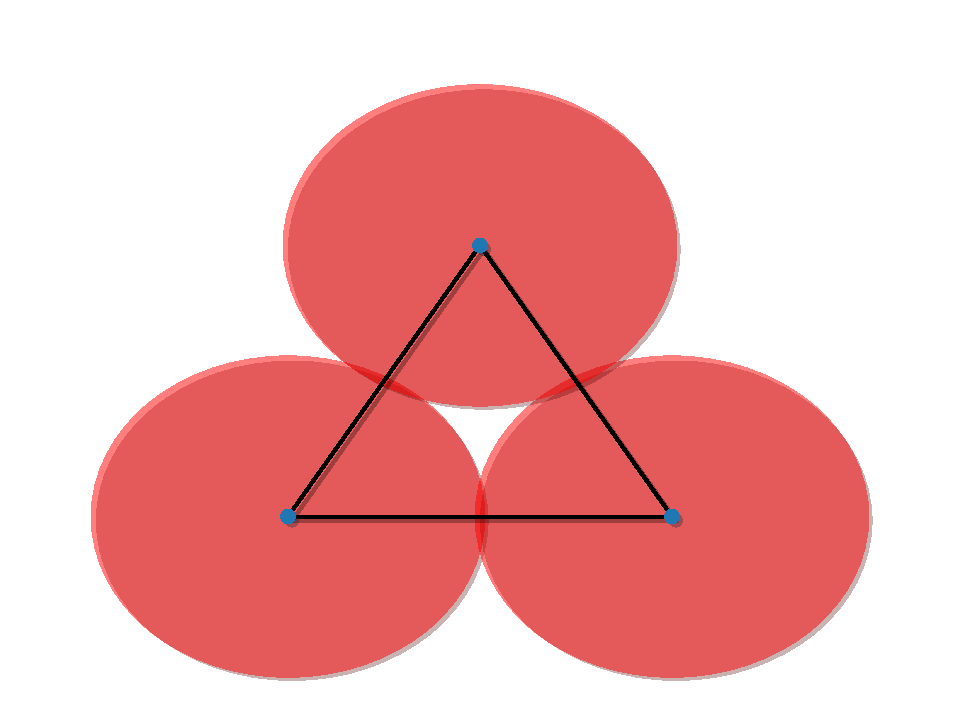
\includegraphics[scale=0.5]{figures/cech1.pdf}
%      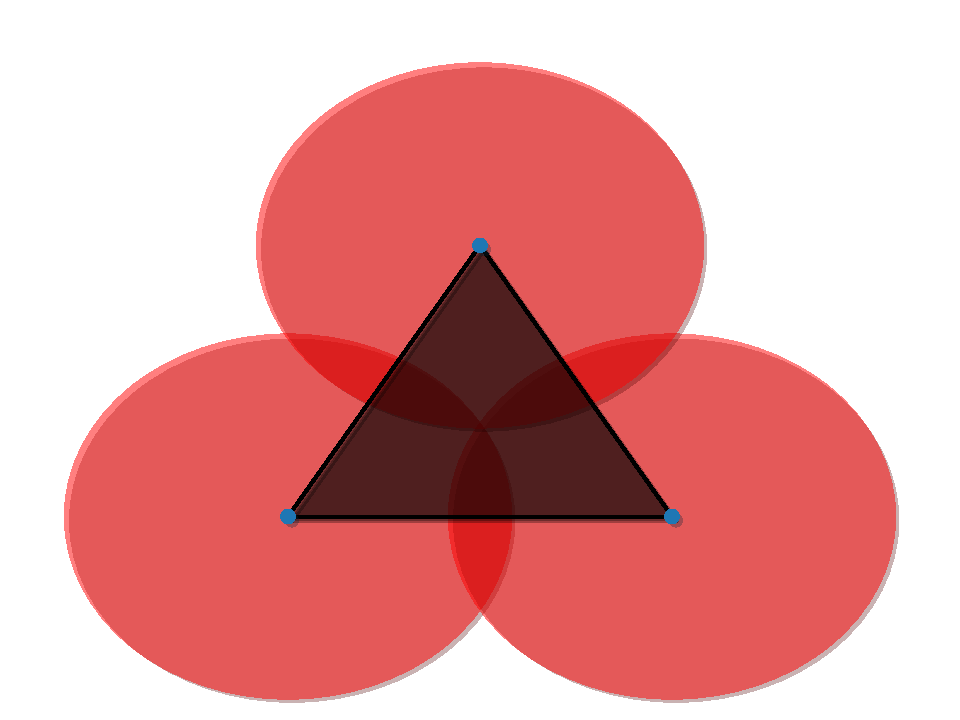
\includegraphics[scale=0.5]{figures/cech2.pdf}
%      \caption{\v Cech complexes of three points at scales $\e, \e'$.}
%      \label{fig:cech}
%  \end{figure}

While the \v Cech complex captures the topology of the coverage region in question exactly it can only be computed when the precise pairwise distances between nodes is known.
If instead we are only provided pairwise \textit{proximity} information indicating when nodes are within some fixed distance we may use the \textbf{(Vietoris-)Rips complex}, defined for a set $P$ at scale $\e > 0$ as
\[ \rips^\e(P) := \left\{\sigma \subseteq P\mid \forall p,q\in\sigma,\ \dist(p, q)\leq\e\right\}. \]

An important result about the relationship of \v Cech and Rips complexes follows from Jung's Theorem~\cite{jung01uber} relating the diameter of a point set $P$ and the radius of the minimum enclosing ball:
\begin{equation}\label{eq:jung_inclusion}
  \cech^\e(P) \subseteq \rips^\e(P) \subseteq \cech^{\jungd \e}(P),
\end{equation}
where the constant $\jungd = \sqrt{\frac{2d}{d+1}}$ (see~\cite{buchet15efficient}).

% \begin{figure}[htbp]
%  \centering
%      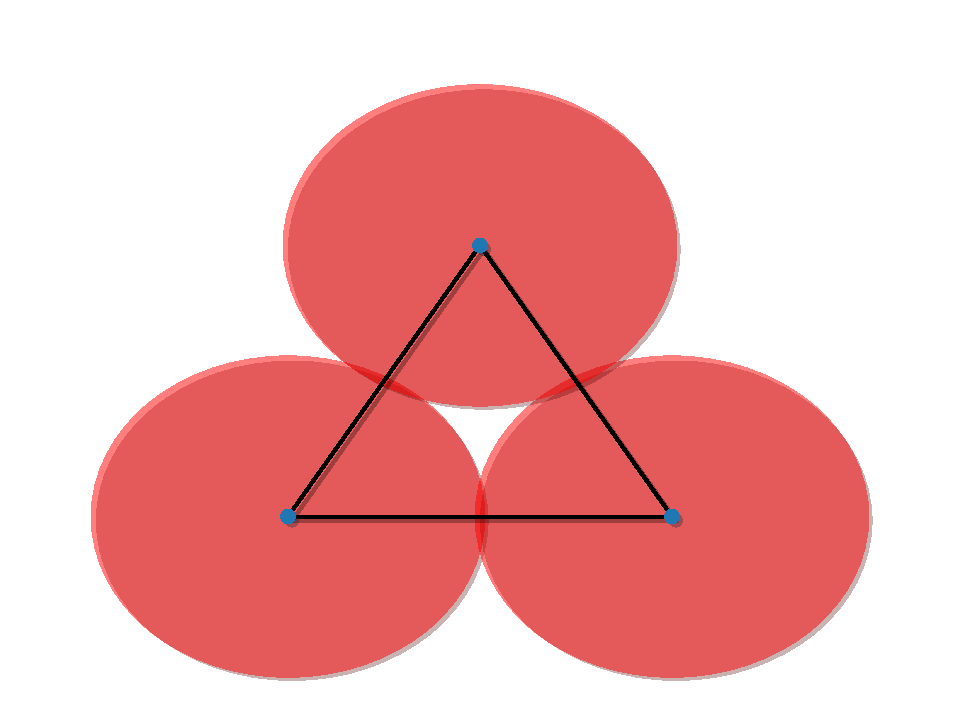
\includegraphics[scale=0.33]{figures/include1.pdf}
%      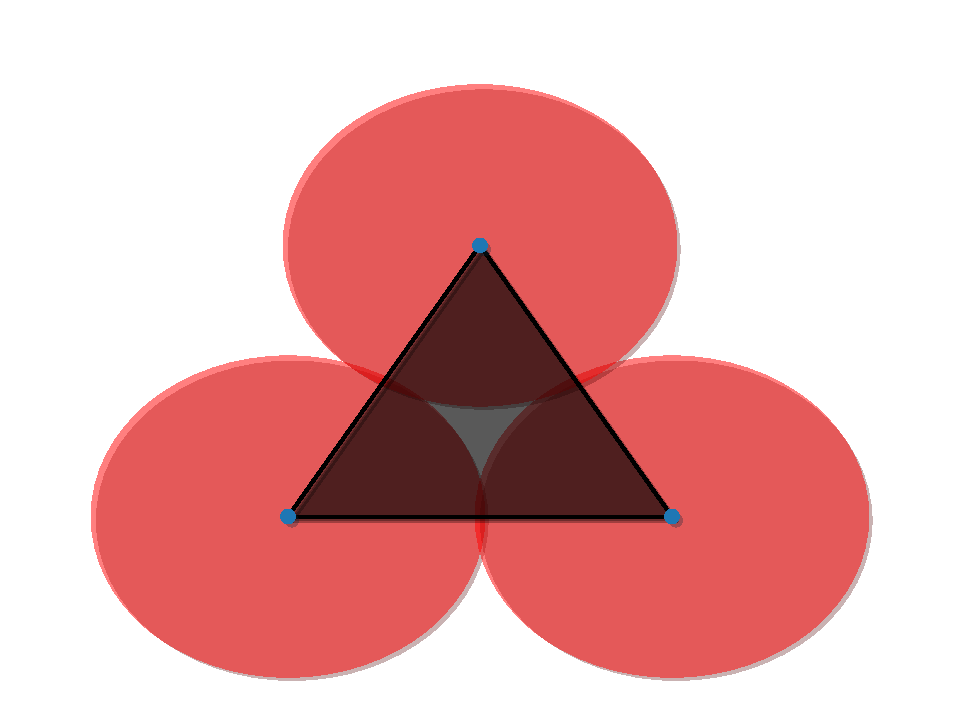
\includegraphics[scale=0.33]{figures/include2.pdf}
%      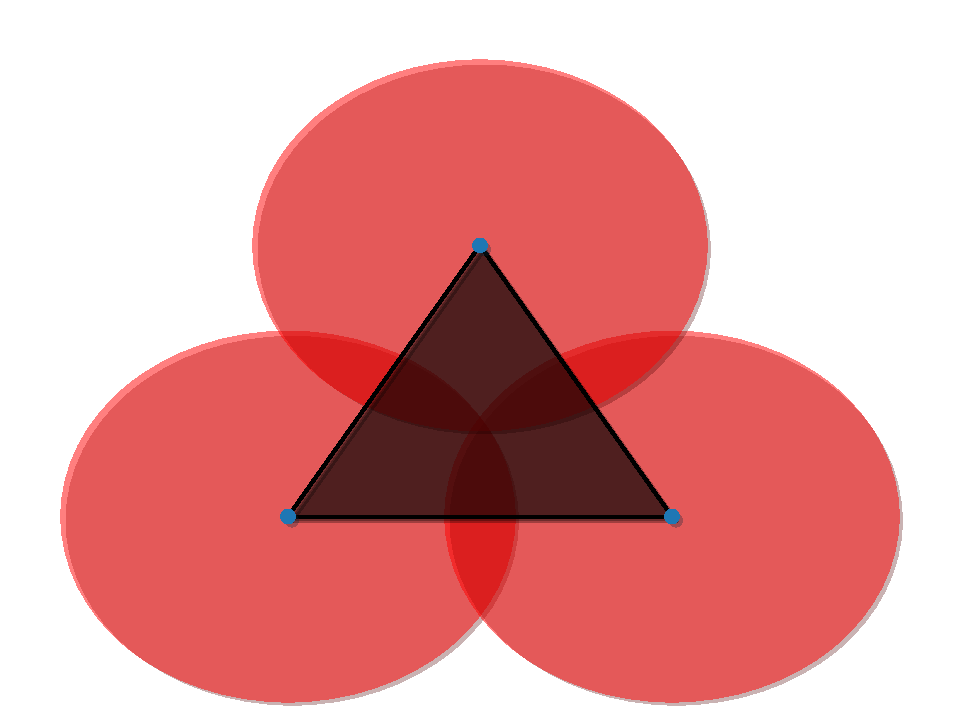
\includegraphics[scale=0.33]{figures/include3.pdf}
%      \caption{The Rips-\v Cech interleaving $\cech^\e(P) \subseteq \rips^\e(P) \subseteq \cech^{\jungd \e}(P)$ }
%      \label{fig:incluson}
%  \end{figure}

As we will see the Rips complex may be used to verify coverage of a domain satisfying some minimal assumptions when we allow the sensors in our network to communicate at two radii $\alpha$ and $\beta$.
In short, if the the inclusion of Rips complexes at scales $\alpha < \beta$ resembles the structure of a subset of the domain then the \v Cech complex at scale $\alpha$, and therefore $P^\alpha$, does as well.

\subsection{Implementation}

\begin{figure}[htbp]
\centering
    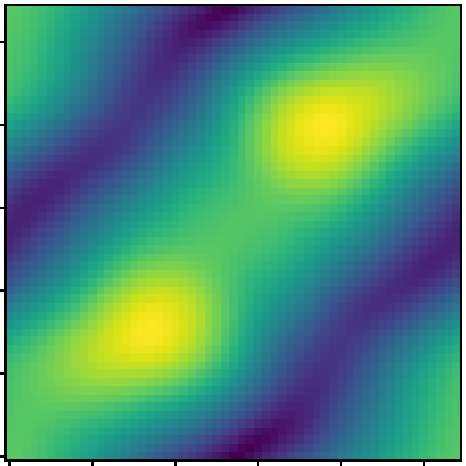
\includegraphics[scale=0.85]{figures/hsn_field.pdf}\hspace{0.5in}
    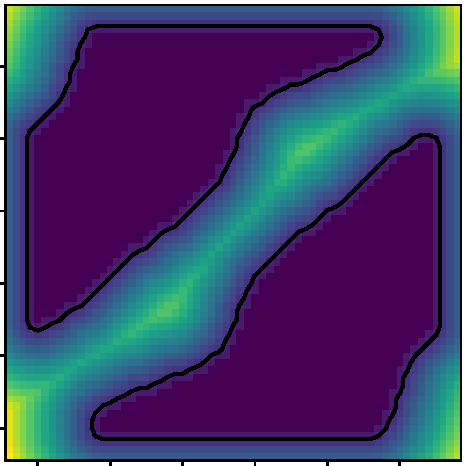
\includegraphics[scale=0.8]{figures/hsn_boundary.pdf}
    \caption{}
    \label{fig:hsn}
\end{figure}

\begin{figure}[htbp]
\centering
    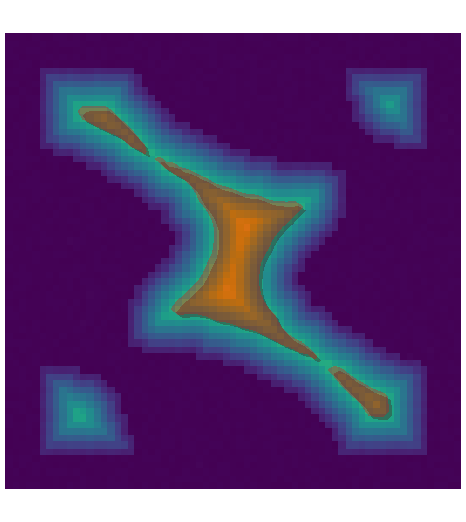
\includegraphics[scale=0.85]{figures/hsn_as1_1.pdf}\hspace{0.5in}
    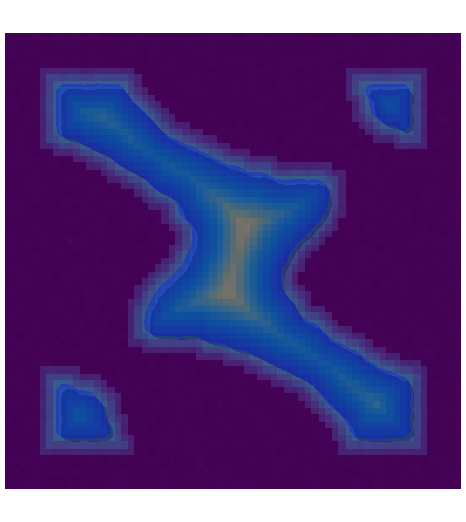
\includegraphics[scale=0.85]{figures/hsn_as1_2.pdf}
    \caption{}
    \label{fig:hsn_as1}
\end{figure}

\begin{figure}[htbp]
\centering
    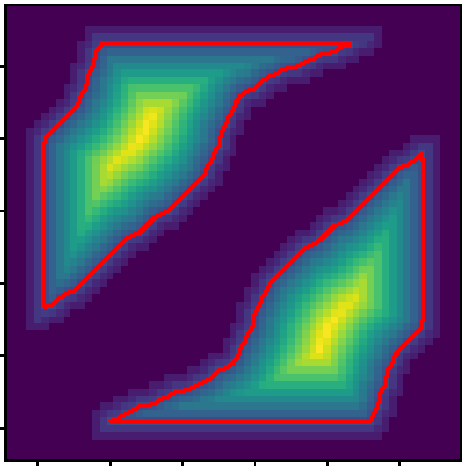
\includegraphics[scale=0.85]{figures/hsn_as2_1.pdf}\hspace{0.5in}
    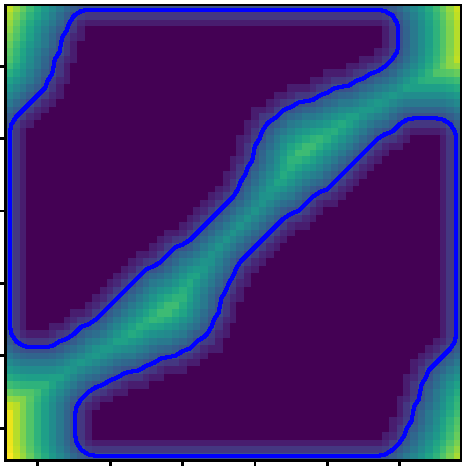
\includegraphics[scale=0.85]{figures/hsn_as2_2.pdf}
     \caption{}
     \label{fig:hsn_as2}
 \end{figure}

 % \begin{figure}[htbp]
 % \centering
 %     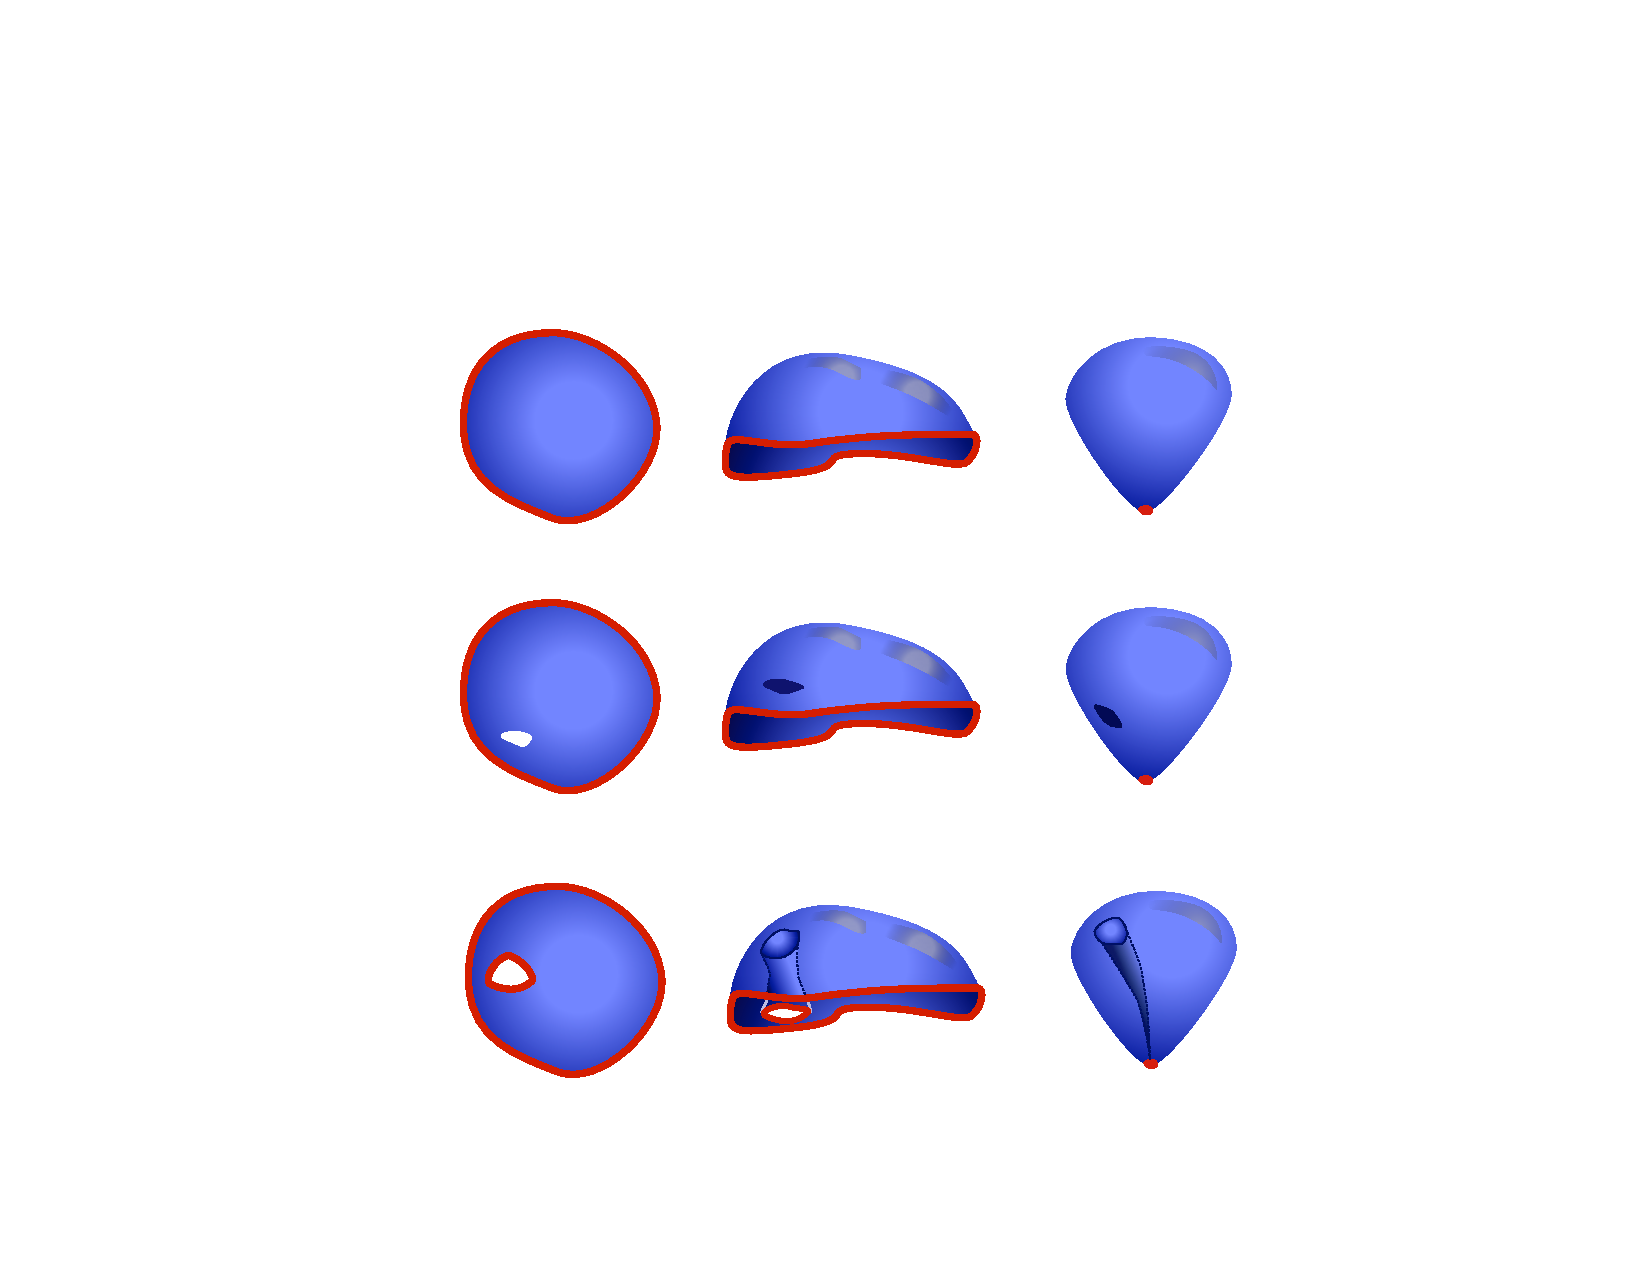
\includegraphics[scale=0.5]{figures/balloons.pdf}
 %      \caption{}
 %      \label{fig:balloons}
 %  \end{figure}

% section tcc (end)
